% Created 2018-03-06 mar 16:38
\documentclass[letterpaper,fleqn]{scrartcl}
\usepackage[utf8]{inputenc}
\usepackage[T1]{fontenc}
\usepackage{fixltx2e}
\usepackage{graphicx}
\usepackage{longtable}
\usepackage{float}
\usepackage{wrapfig}
\usepackage{rotating}
\usepackage[normalem]{ulem}
\usepackage{amsmath}
\usepackage{textcomp}
\usepackage{marvosym}
\usepackage{wasysym}
\usepackage{amssymb}
\usepackage{hyperref}
\tolerance=1000
\usepackage{khpreamble}
\usepackage{tabularx}
\usepackage{geometry}
\usepackage{pgfplots}
\pgfplotsset{compat=1.13}
\geometry{top=20mm, bottom=20mm, left=24mm, right=18mm}
\author{Kjartan Halvorsen}
\date{}
\title{State feedback exercise}
\hypersetup{
  pdfkeywords={},
  pdfsubject={},
  pdfcreator={Emacs 24.5.1 (Org mode 8.2.10)}}
\begin{document}

\maketitle

\section*{Input signal design}
\label{sec-1}
Consider the sampled double-integrator on state-space form
\begin{equation}
\begin{aligned}
x(kh+h) &= \underbrace{\bbm 1 & h\\ 0 & 1\ebm}_{\Phi(h)} x(kh) + \underbrace{\bbm \frac{h^2}{2}\\h\ebm}_{\Gamma(h)} u(kh)\\
y(kh) &= \bbm 1 & 0 \ebm x(kh)
\end{aligned}
\label{eq:ss}
\end{equation}
We want to find the input sequence $u(0)$, $u(h)$ that takes the system from the origin of the state space $x(0) = \bbm 0 & 0 \ebm\transp$ to the point $x(2h) = \bbm a & 0 \ebm\transp$ in two time steps. 

\subsection*{Iterate the state space model}
\label{sec-1-1}
\ldots{} in order to find an expression for $x(2h)$ in terms of the unknown input signals
\begin{align*}
x(h) &= \Phi x(0) + \Gamma u(0) \\
x(2h) &= \Phi x(h) + \Gamma u(h) = \Phi\left(\Phi x(0) + \Gamma u(0)\right) + \Gamma u(h)\\
          &= \Phi^2x(0) + \Phi\Gamma u(0) + \Gamma u(h)
          = \Phi^2x(0) + \underbrace{\bbm & & & & \ebm}_{W_c} \bbm u(h)\\u(0) \ebm  
\end{align*}

\subsection*{Set up system of equations}
\label{sec-1-2}
With \(u = \bbm u(h) & u(0) \ebm\transp\) we get the linear system of equations \(W_c u = x(2)-\Phi^2x(0)\). In the particular case we are considering here this gives
\[ \bbm & & & & &\\ & & & & &\\ & & & & & \ebm \bbm u(h)\\u(0)\ebm = \bbm & &  \\ && \\ &&\ebm.\]


\newpage

\section*{Verify the result}
\label{sec-2}

\subsection*{Calculate the state sequence}
\label{sec-2-1}
\begin{align*}
x(h) &= \\
x(2h) &= 
\end{align*}

\subsection*{Plot the results}
\label{sec-2-2}
\begin{center}
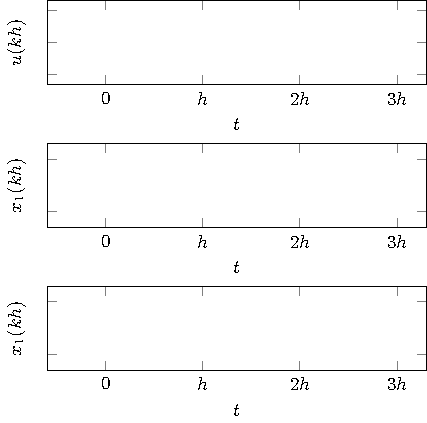
\includegraphics[width=0.6\linewidth]{../figures/empty-input-state-sequences}
\end{center}

\section*{The deadbeat control law}
\label{sec-3}
We are looking for the linear control law \(u(kh) = l_0y_{ref}(kh) - Lx(kh) = l_0y_{ref}(kh) - l_1x_1(kh) -l_2x_2(kh)\) that produced the result above.
\subsection*{Set up the equations}
\label{sec-3-1}
\begin{description}
\item[{\(k=0\):}] \(u(0) = \)
\item[{\(k=1\):}] \(u(h) = \)
\item[{\(k=2\):}] \(u(2h) = \)
\end{description}

\subsection*{Solve the system of equations}
\label{sec-3-2}
Write the system of equations

\[ \bbm & & & & & & & &\\ & & & & & & & &\\ & & & & & & & & \\ & & & & & & & &  \ebm \bbm l_0\\l_1\\l_2\ebm = \bbm && &  \\ &&& \\ &&& \\ && &\ebm.\]

\newpage

\subsection*{The poles of the closed-loop system}
\label{sec-3-3}

Inserting the control law \(u(kh) = l_0y_{ref}(kh) - Lx(kh)\) into the state-space system \eqref{eq:ss} gives the closed-loop system
\begin{equation*}
\begin{aligned}
 x(kh+h) &= \Phi x(kh) + \Gamma u(kh) = \Phi x(kh) - \Gamma L x(kh) + \Gamma l_0y_{ref}(kh)\\
    &= \\
\end{aligned}
\end{equation*}

Determine the poles of the closed-loop system.
% Emacs 24.5.1 (Org mode 8.2.10)
\end{document}